\section{Бутстреп оценка стандартной ошибки}

Бутстреп методы зависят от понятия бутстреп выборки. Пусть $\hat F$ -- эмпирическое распределение, присваивающее вероятность $1 / n$ на каждое из наблюдаемых значений $x_i$, $i = 1, 2,\cdots, n$, как описано в главе 4. Бутстреп выборка является случайной выборкой размера $n$, набранной из $\hat F$, скажем, $\mathbf{x}^* = (x_1^*, x_2^*, \cdots, x_n^*)$,
\begin{equation}
    \hat F\rightarrow (x_1^*, x_2^*, \cdots, x_n^*).
\end{equation}
<<*>> указывает, что $\mathbf{x}^*$ не является фактическим набором данных $\mathbf{x}$, а скорее рандомизированной или перезапущенной версией $\mathbf{x}$.

Есть еще один способ сказать (6.1): точки бутстреп данных $x_1^*, x_2^*, \cdots, x_n^*$ являются случайной выборкой размера $n$, выбранной с заменой из совокупности $n$ объектов $(x_1, x_2, \cdots, x_n )$. Таким образом, мы могли бы иметь $x_1^* = x_7, x_2^* = x_3, x_4^* = x_3, x_4^* = x_{22},\cdots, x_n^* = x_7$. Набор бутстреп данных $(x_1^*, x_2^*, \cdots, x_n^*)$ состоит из элементов исходного набора данных $(x_1, x_2,\cdots, x_n)$, некоторые из которых появляются ноль раз, некоторые появляются один раз, некоторые появляются дважды, и так далее.

В соответствии с набором бутстреп данных $\mathbf{x}^*$, бутстреп репликация $\hat\theta$ -- это
\begin{equation}
    \hat\theta^*=s(\mathbf{x}^*).
\end{equation}
Величина $s(\mathbf{x}^*)$ является результатом применения той же функции $s (\cdot)$ к $\mathbf{x}^*$, которая была применена к $\mathbf{x}$. Например, если $s(\mathbf{x})$ является выборочным средним значением $\bar x$, то $s(\mathbf{x}^*)$ -- это среднее значение набора бутстреп данных, $\bar x^*=\sum_{i=1}^nx_i^*/n$. 

Бутстреп оценка $se_F (\hat\theta)$ стандартной ошибки статистики $\hat\theta$ представляет собой плагин оценку, которая использует эмпирическую функцию распространения $\hat F$ вместо неизвестного распределения $F$. В частности, бутстреп оценка  $se_F (\hat\theta)$ определяется, как 
\begin{equation}
    se_{\hat F} (\hat\theta^*).
\end{equation}
Другими словами, бутстреп оценка $se_F (\hat\theta)$ является стандартной ошибкой $\hat\theta$ для наборов данных размером $n$, случайным образом выбранных из $\hat F$. 

Формула (6.3) называется идеальной бутстреп оценкой ошибки $\hat\theta$. К сожалению, для практически любой оценки $\hat\theta$, кроме среднего, нет точной формулы (5.4), которая позволяет вычислить числовое значение идеальной оценки точно. Бутстреп алгоритм, описанный ниже, является вычислительным способом получения хорошего приближения к численному значению $se_{\hat F} (\hat\theta^*)$. 

Легко реализовать бутстреп выборку на компьютере. Устройство выбирает случайные целые числа $i_1, i_2, \cdots, i_n$, каждое из которых равняется любому значению между 1 и $n$ с вероятностью $1 / n$. Бутстреп выборка состоит из соответствующих членов $\mathbf{x}$,
\begin{equation}
    x_1^*=x_{i_1},x_2^*=x_{i_2},\cdots,x_n^*=x_{i_n}.
\end{equation}

Бутстреп алгоритм работает путем выбора множества независимых бутстреп выборок, оценки соответствующих бутстреп репликаций и оценки стандартной ошибки $\hat\theta$ через эмпирическое стандартное отклонения репликаций. Результат называется бутстреп оценкой стандартной ошибки, обозначенной $\widehat{se}_B$, где $B$ -- количество используемых бутстреп выборок.

Алгоритм 6.1 -- это более явное описание бустреп процедуры для оценки стандартной ошибки $\hat\theta=s(\mathbf{x})$ из наблюдаемых данных $\mathbf{x}$. 

\newpage
\begin{center}
    \textit{Алгоритм 6.1}
    
    \underline{Бутстреп алгоритм для оценки стандартных ошибок}
    
    \begin{enumerate}
        \item Выберите $B$ независимых бутстреп выборок $x^{*1}, x^{*2},\cdots, x^{*B}$, каждый из которых состоит из $n$ точек данных, выбранных с заменой их $\mathbf{x}$, как в (6.1) или (6.4). [Для оценки стандартной ошибки B обычно будет в диапазоне 25-200, см. Таблицу 6.1.] 
        
        \item Оцените бутстреп репликацию, соответствующую каждой бутстреп выборке,
        \begin{equation}
            \hat\theta^*(b)=s(\mathbf{x}^{*b})\qquad b=1,2,\cdots,B.
        \end{equation}
        
        \item Оцените стандартную ошибку $se_F (\hat\theta)$ через выборочное стандартное отклонение $B$ репликаций 
        \begin{equation}
            \widehat{se}_B=\left\{\sum_{b=1}^B[\hat\theta^*(b)-\hat\theta^*(\cdot)]^2/(B-1)\right\}^{1/2},
        \end{equation}
        где $\hat\theta^*(\cdot)=\sum_{b=1}^B\hat\theta^*(b)/B$.
    \end{enumerate}
\end{center}

На рисунке 6.1 изображена схематическая диаграмма бутстреп алгоритма стандартных ошибок. 

Предел $\widehat{se}_B$ по $B$ стремится к бесконечности -- это идеальная бутстреп оценка $se_F(\hat\theta)$,
\begin{equation}
    \lim_{B\rightarrow\infty}\widehat{se}_B=se_{\hat F}=se_{\hat F}(\hat\theta^*).
\end{equation}
Тот факт, что $\widehat{se}_B$ стремится к $se_{\hat F}$ при $B$, стремящимся к бесконечности, позволяет сказать, что эмпирическое стандартное отклонение приближается к стандартному отклонению совокупности с увеличением количества репликаций. «Совокупность» в этом случае является совокупностью значений $\hat\theta^*=s(\mathbf{x}^*)$, где $\hat F \rightarrow (x_1^*, x_2^*, \cdots, x_n^*) = \mathbf{x}^*$. 

Идеальная бутстреп оценка $se_{\hat F}\hat\theta^*$ и его приближение $\widehat{se}_B$ иногда называют непараметрическими бутстреп оценками, потому что они основаны на $\hat F$, непараметрической оценке $F$. В разделе 6.5 мы обсуждим параметрический бутстреп, который использует другую оценку F. 

Немного об обозначениях: в (6.7) мы пишем $se_{\hat F}(\hat\theta^*)$, а не $se_{\hat F}(\hat\theta)$, чтобы избежать путаницы между $\hat\theta$, значением $s (\mathbf{x})$ на основе наблюдаемых данных, и $\hat\theta^* = s (\mathbf{x}^*)$, случайной величиной на основе бутстреп выборки. Более подробное обозначение $se_{\hat F} (\hat\theta (\mathbf{x}^*))$ подчеркивает, что $se_{\hat F}$ является бутстрепированной стандартной ошибкой: фактические данные $\mathbf{x}$ остаются фиксированным в (6.7); Случайность в расчете исходит из изменчивости бутстреп выборок $\mathbf{x}^*$ для данного x. Точно так же мы будем писать $E_{\hat F}g(\mathbf{x^*})$, чтобы указать бутстрепированное математическое ожидание функции $g (\mathbf{x}^*)$: математическое ожидание с фиксированным $\mathbf{x}$ (и $\hat F$) и случайным $\mathbf{x}^*$ в соответствии с (6.1). 
\newline

\noindent
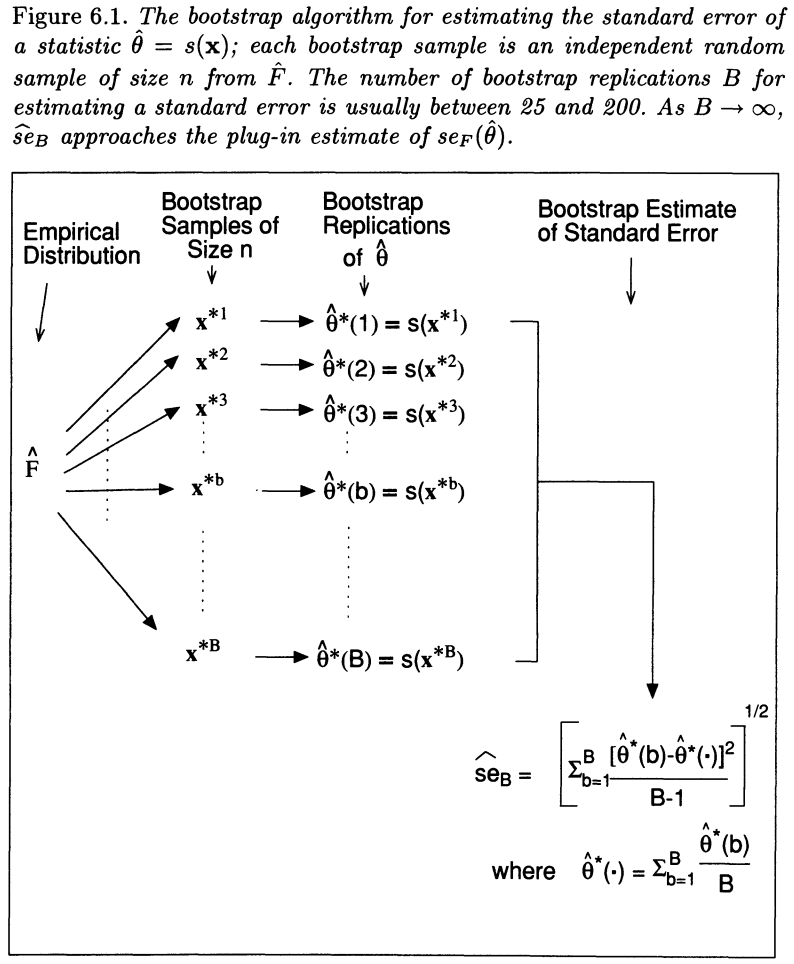
\includegraphics[width=\linewidth]{5/f61.png}
\newline

Всего существует $C_n^{2n-1}$ различных бутстреп выборок. Обозначим их через $z^1, z^2, \ldots z^m$, где $m = C_n^{2n-1}$. Например, если $n = 2$, отдельными выборками являются $(x_1, x_1)$, $(x_2, x_2)$ и $(x_1, x_2)$; поскольку порядок не имеет значения, $(x_2, x_1)$ совпадает с $(x_1, x_2)$. Вероятность получения одной из этих выборок при выборе с заменой может быть получена из полиномиального распределения. Обозначим вероятность $j$-й выборки через $\omega_j, j = 1, 2, \ldots C_n^{2n-1}$. Тогда прямым способом вычисления идеальной бутстреп оценки стандартной ошибки будет использование стандартного отклонения совокупности m бутстреп значений $s (z^j)$:
\begin{equation}
    se_{\hat F}(\hat\theta^*)=[\sum_{j=1}^m\omega_j\{s(z^j)-s(\cdot)\}^2]^{1/2}
\end{equation}
где $s (\cdot) = \sum_{j=1}^m\omega_js(z^j)$. Сложность этого подхода заключается в том, что, если $n$ не достаточно мало $(\le 5)$, число $C_n^{2n-1}$ очень велико, что делает вычисление (6.8) непрактичным. Отсюда необходимость в бутстрап выборкaх, описаных выше. 